\appendix
\section{Kuno's Conjecture \label{appendix1}}
For a given triplet, the sum of the channel number of each cluster will be a constant.
 

% \begin{figure}[h!]
  %\begin{center}
     % 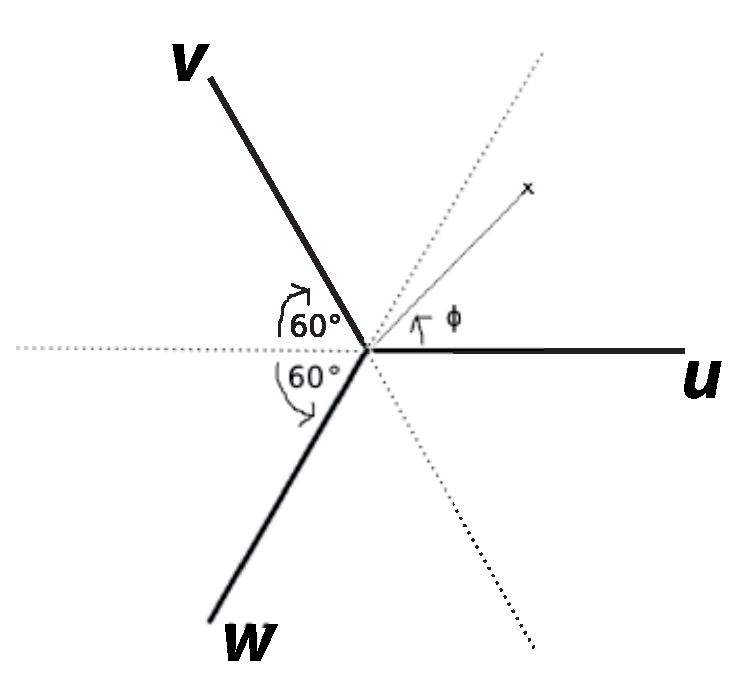
\includegraphics[scale=0.6]{figures/kuno.eps}
    %  \end{center}
    %  \caption{Schematic representation of a point and the three plane orientations.}
      % \label{hjj}
%\end{figure}

 Considering that the u axis parallel to x,
 
 \[
 \mbox{u}=\mbox{r}\cos\theta
 \]
 \[
 \mbox{v}=\mbox{r}\cos \left [ \frac{2\pi}{3}-\phi \right ]
 \]
 \[
 \mbox{w}=\mbox{r}\cos \left [\frac{4\pi}{3}-\phi \right ]
 \]
 
 So, one can write:
 
\begin{eqnarray}
\mbox{u}+\mbox{v}+\mbox{w} &=& r \left [ \cos \phi + \cos \left [ \frac{2\pi}{3}-\phi \right ] + \cos \left [\frac{4\pi}{3}-\phi \right ] \right] \\
                &=& 0
\end{eqnarray}

In the case when the centre of the station is not the origin of the reference frame, the sum of the the three views will equal the sum of the central fibres number: $106.5+106.5+105.5 = 318.5$. The following figure shows the sum of channel numbers for a random collection of space-points retrieved from G4MICE. The bins 318 and 319 share the counts we expected to see.
 
 \begin{figure}[h!]
  \begin{center}
      \includegraphics[scale=0.7]{figures/Ch_sum.eps}
      \end{center}
      \caption{.}
       \label{some}
\end{figure}

\section{Space-Points Standard Deviation \label{appendix2}}
Figure \ref{drawing} shows the disposal of the fibres in the tracker. 
\begin{figure}[h!]
  \begin{center}
      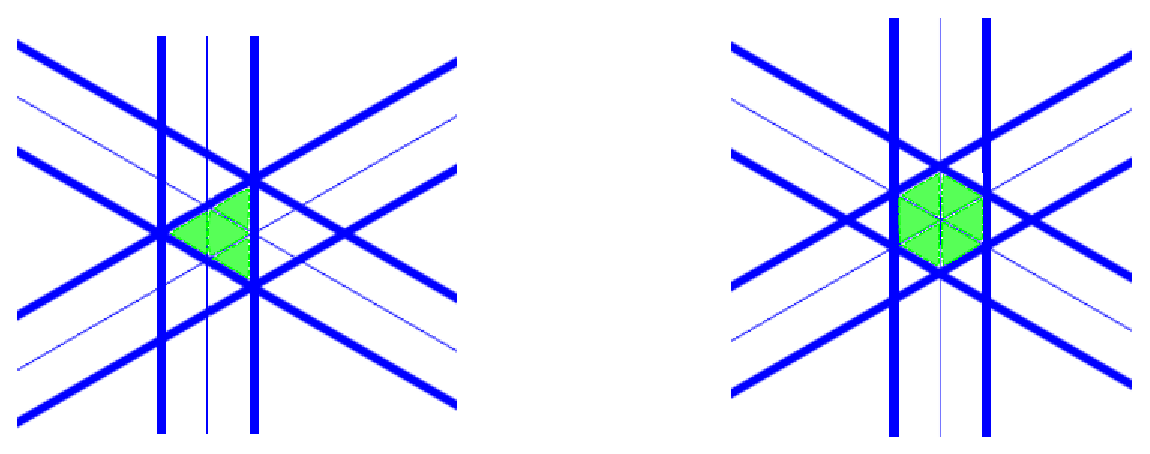
\includegraphics[scale=0.7]{figures/drawing2.eps}
      \end{center}
      \caption{\textsc{Right:} fibre arrangement in station 5 of tracker 1. \textsc{Left:} Fibre arrangement in the rest of the stations. As it is shown by the green areas, the intersection of the three channels array will be a triangle for every station except for station 5, where it will be an hexagon.}
       \label{drawing}
\end{figure}

For the triangular intersection, the mean values of x and y are:

\begin{eqnarray}
 \bar{x} &=& \frac{1}{A} \int \int x dx dy  = \frac{1}{A}  \int_{0}^{\omega} x dx \int_{-\frac{x}{\sqrt{3}}}^{\frac{x}{\sqrt{3}}} dy = \frac{1}{A}  \int_{0}^{\omega} \frac{2 x^{2}}{\sqrt{3}} dx = \frac{1}{A} \frac{2\omega^{3}}{3\sqrt{3}} = \frac{2}{\sqrt{3}} \frac{\omega^{3} \sqrt{3}}{3\omega^{2}} \nonumber \\
   &=& \frac{2}{3}\omega  \nonumber \\
\end{eqnarray}

\begin{eqnarray}
 \bar{y} &=& \frac{1}{A} \int \int y dx dy  = \frac{1}{A}  \int_{0}^{\omega} dx \int_{-\frac{x}{\sqrt{3}}}^{\frac{x}{\sqrt{3}}} y dy = \frac{1}{A}  \int_{0}^{\omega} \left[ \frac{y^{2}}{2} \right]_{-\frac{x}{\sqrt{3}}}^{\frac{x}{\sqrt{3}}} dx \nonumber \\
   &=& 0 % \nonumber \\
\end{eqnarray}


from which the RMS values can be calculated:

\begin{eqnarray}
[RMS_{x}]^{2} &=& \frac{1}{A} \int \int (x-\bar{x})^{2} dx dy = \frac{1}{A} \int_{0}^{\omega} dx \int_{-\frac{x}{\sqrt{3}}}^{\frac{x}{\sqrt{3}}}  (x-\bar{x})^{2} dy = \frac{1}{A} \frac{2}{\sqrt{3}} \int_{0}^{\omega} x (x-\bar{x})^{2} \nonumber \\
   &=& \frac{1}{A} \frac{2}{\sqrt{3}} \int_{0}^{\omega} x^{3}-x^{2}\bar{x}+\bar{x}^{2}x dx = \frac{1}{A} \frac{2}{\sqrt{3}} \int_{0}^{\omega} x^{3}-\frac{4}{3}\omega x^{2}+ \frac{4}{9} \omega^{2} x dx  \nonumber \\
   &=& \frac{1}{A} \frac{2}{\sqrt{3}} \left[ \frac{x^{4}}{4} - \frac{4\omega}{9}x^{3} + \frac{2\omega^{2}}{9}x^{2}\right]_{0}^{\omega} = \omega^{2} \left(  \frac{1}{2}-\frac{4}{9} \right) = \frac{\omega^{2}}{3\sqrt{2}}
\end{eqnarray}

\begin{eqnarray}
[RMS_{y}]^{2} &=& \frac{1}{A} \int_{0}^{\omega} dx \int_{-\frac{x}{\sqrt{3}}}^{\frac{x}{\sqrt{3}}}(y-\bar{y})^{2} dy = \frac{1}{A} \int_{0}^{\omega} \left[ \frac{y^{3}}{3} \right]_{-\frac{x}{\sqrt{3}}}^{\frac{x}{\sqrt{3}}} dy =  \frac{1}{A} \frac{2}{3^{\frac{5}{2}}} \int_{0}^{\omega} x^{3}dx \nonumber \\
   &=& \frac{2\sqrt{3}}{\omega^{2}3^{\frac{5}{2}}} \left[ \frac{x^{4}}{4} \right]_{0}^{\omega} = \frac{\omega^{2}}{3\sqrt{2}} 
\end{eqnarray}

So, 
\[
\sigma_{x}=\sigma_{y}=\frac{\omega}{3\sqrt{2}} = 384.4 \unit{\mu m}
\]

For the hexagonal case:
The area of the overlapping region (shaded zone in figure \ref{} right)
\begin{eqnarray}
A=6\times\frac{1}{2}\times \frac{\omega}{\sqrt{3}}\times \frac{\omega}{2}=\frac{\sqrt{3}}{2}\omega^{2}
\end{eqnarray}

\begin{eqnarray}
[RMS_{x}]^{2} &=& \frac{1}{A} \int \int (x-\bar{x})^{2} dx dy = \frac{2}{A}  \int_{-\frac{\omega}{2}}^{0}x^{2} dx \int_{-\frac{x}{\sqrt{3}}-\frac{\omega}{\sqrt{3}}}^{\frac{x}{\sqrt{3}}+\frac{\omega}{\sqrt{3}}} dy \nonumber \\
&=& \frac{2}{A}\int_{-\frac{\omega}{2}}^{0}x^{2} \rigth[ \frac{x}{\sqrt{3}}+\frac{\omega}{\sqrt{3}}  \left ] dx = \frac{4}{A\sqrt{3}}\int_{-\frac{\omega}{2}}^{0} \rigth ( x^{3}+ x^{2}\omega \left )dx \nonumber \\
&=& \frac{4}{A\sqrt{3}} \rigth [ -\frac{1}{4}\frac{\omega^{4}}{16}+\frac{1}{3}\frac{1}{8}\omega^{4}\left ] = \frac{\omega^{4}}{2A\sqrt{3}} \rigth[ \frac{1}{3}-\frac{1}{8} \left] \nonumber \\
&=& \frac{5\omega^{4}}{16.3.\sqrt{3}}\frac{2}{\sqrt{3}\omega^{2}} = \sqrt{{5}{2}}\frac{\omega}{6}=429.8 \unit{\mu m}
\end{eqnarray}

\section{Straight Track Pattern Recognition \label{appendix4}}
An example of the method for the case where space points are confined in three
statins are given below
1- The routine finds the slopes of the line in the $x-z$ plane and $y-z$ plane
using the space points $1$ and $3$

\begin{equation}
\begin{split}
m_x=\frac{x_{1}-x{3}}{z_{1}-z_{3}}\\
m_y=\frac{y_{1}-y{3}}{z_{1}-z_{3}}
\end{split}
\end{equation}

Equations of the line passing through the first and the last
points would read

\begin{equation}
\begin{split}
(x-x_{1}) &=m_{x}(z-z_{1})\\
(y-y_{1}) &=m_{y}(z-z_{1})
\end{split}
\end{equation}

an ideal case would happen if the coordinates of the space
point $2$ can satisfy the above equations
\begin{equation}
\begin{split}
(x_{2}-x_{1}) &=m_{x}(z_{2}-z_{1})\\
(y_{2}-y_{1}) &=m_{y}(z_{2}-z_{1})
\end{split}
\end{equation}

but more likely the line does not pass through the space point in station 2
and there would be some $\Delta_{x_2}$ and $\Delta_{y_2}$ deviations
\begin{equation}
\begin{split}
(x-x_{1}) &=m_{x}(z-z_{1})\\
(y-y_{1}) &=m_{y}(z-z_{1})
\end{split}
\end{equation}
\begin{equation}
\begin{split}
\Delta_{x_2} &=m_{x}(z_{2}-z_{1})-(x_{2}-x_{1})\\
\Delta_{y_2} &=m_{y}(z_{2}-z_{1})-(y_{2}-y_{1})
\end{split}
\end{equation}
It is a common practice to accept the line equations if
$\Delta_{x_2}$ and $\Delta_{y_2}$ deviations  remain within  
 predefined values like 
$|\Delta_{x_2}|< 15 \text{mm}$  and  $|\Delta_{y_2}|<15 \text{mm}$.
 
If the routine finds four space points relating to 4 stations,
again the slopes of the line passing through the 
the first and the last points in $x-z$ and $y-z$ would be

\begin{equation}
\begin{split}
m_x=\frac{x_{1}-x_{4}}{z_{1}-z_{4}}\\
m_y=\frac{y_{1}-y_{4}}{z_{1}-z_{4}}
\end{split}
\end{equation}

 and equations of the line

\begin{equation}
\begin{split}
(x-x_{1}) &=m_{x}(z-z_{1})\\
(y-y_{1}) &=m_{y}(z-z_{1})
\end{split}
\end{equation}

if the coordinates of the space points $2$ and $3$ satisfy the above
equations
\begin{equation}
\begin{split}
(x_{2}-x_{1}) &=m_{x}(z_{2}-z_{1})\\
(y_{2}-y_{1}) &=m_{y}(z_{2}-z_{1})\\
(x_{3}-x_{1}) &=m_{x}(z_{3}-z_{1})\\
(y_{3}-y_{1}) &=m_{y}(z_{3}-z_{1})
\end{split}
\end{equation}

we have an ideal case, but a more portable case would produce 
some $\Delta_{x}$ and $\Delta_{y}$ deviations
\begin{equation}
\begin{split}
\Delta_{x_2} &=(x_{2}-x_{1})- m_{x}(z_{2}-z_{1})\\
\Delta_{y_2} &=(y_{2}-y_{1})-m_{y}(z_{2}-z_{1})\\
\Delta_{x_3} &=(x_{3}-x_{1})-m_{x}(z_{3}-z_{1})\\
\Delta_{y_3} &=(y_{3}-y_{1})- m_{y}(z_{3}-z_{1})
\end{split}
\end{equation}
Small deviation values $|\Delta_{x_{1,2}}|<15 ~\text{mm}$ 
 and $|\Delta_{y_{1,2}}|<15 ~\text{mm}$  may still be acceptable.
The generalisation of the forgoing method to $5$
space points will be straightforward. 

\section{Helical Track Pattern Recognition \label{appendix4}}
The equation of motion of a charged particle in an external magnetic field
can be written as

\begin{equation}
\frac{d^2 x}{ds^2}=\frac{q}{p}(\frac{d \vec{x}}{ds})\times \vec{B}(s)
\end{equation}
If we assume that the magnetic filed lies along the $z$ axis $\vec{B}=(0,0,B)$
, then the three scaler components of it can be wirttien as
\begin{equation}
\begin{split}
\frac{d^2 x}{ds^2} &=\frac{q}{P}(\frac{dy}{ds})B\\
\frac{d^2 y}{ds^2} &=-\frac{q}{P}(\frac{dx}{ds})B\\
\frac{d^2 z}{ds^2} &=0
\end{split}
\end{equation}

we also note that $P$ is the total momentum and the transverse
momenumte $p_t =P \cos \lambda=qBR_H$
can be written as

\begin{equation}
\begin{split}
p_x &=p_t \cos \phi\\
p_x &=-p_t \sin \phi
\end{split}
\end{equation}

the solution of the above equations will be a helix

\begin{equation}
\begin{split}
x(s) &=x_{1} + R \left[\cos \left(\Phi_{0}+\frac{hs\cos \lambda}{R} \right)-\cos \Phi_{0} \right]\\
y(s) &=y_{1} + R \left[\cos \left(\Phi_{0}+\frac{hs\cos \lambda}{R} \right)-\sin \Phi_{0} \right]\\
z(s) &=z_{1}+s \sin \lambda
\end{split}
\end{equation}

where $x_{1}$, $y_{1}$ and $z_{1}$ is the starting point. $R$ is the radius of the helix.
$h=\pm 1$ is the sense of the rotation in $x-y$ plane. We note that
\begin{equation}
 \begin{split}
ds^2 =dx^2+dy^2+dz^2\\
ds/dz =(1+\acute{x}^2+\acute{y}^2)^{1/2}\\
(\frac{dx}{ds})^2 +(\frac{dy}{ds})^2 + (\frac{dz}{ds})^2 = 1
\end{split}
\end{equation}



On the other hand, the equation of a circle passing through three space points $(x_i,y_i)$ , where
$i=1,2,3$ can be found from the following determinant.

\begin{equation}
\left|
\begin{matrix}
x^2+y^2 & x & y & 1\\
x_1^2+y_1^2 & x_1 & y_1 & 1\\
x_2^2+y_2^2 & x_2 & y_2 & 1\\
x_3^2+y_3^3 & x_3 & y_3  & 1
\end{matrix}
\right|
=0
\end{equation}
which can be re-written as
\begin{equation}
(x^2+y^2)
\left|
\begin{matrix}
 x_1 & y_1 & 1\\
 x_2 & y_2 & 1\\
 x_3 & y_3 & 1
\end{matrix}
\right|
-x
\left|
\begin{matrix}
x_1^2+y_1^2 & y_1 & 1\\
x_2^2+y_2^2 & y_2 & 1\\
x_3^2+y_3^3 & y_3  & 1
\end{matrix}
\right|
+y
\left|
\begin{matrix}
x_1^2+y_1^2 & x_1 & 1\\
x_2^2+y_2^2 & x_2 & 1\\
x_3^2+y_3^3 & x_3 & 1
\end{matrix}
\right|
-
\left|
\begin{matrix}
x_1^2+y_1^2 & x_1 & y_1 \\
x_2^2+y_2^2 & x_2 & y_2 \\
x_3^2+y_3^3 & x_3 & y_3
\end{matrix}
\right|
=0
\end{equation}

comparing the above relation with the conventional circle equation
\begin{equation}
a(x^2+y^2)+dx+ey+f=0
\end{equation}
or
\begin{equation}
(x+\frac{d}{2a})^2+(y+\frac{e}{2a})^2=\left( \sqrt{\frac{d^2+e^2}{4a^2}-\frac{f}{a} } \right)^2
\end{equation}
we find that


\begin{equation}
a=
\left|
\begin{matrix}
 x_1 & y_1 & 1\\
 x_2 & y_2 & 1\\
 x_3 & y_3 & 1
\end{matrix}
\right|
\end{equation}

\begin{equation}
d=-
\left|
\begin{matrix}
x_1^2+y_1^2 & y_1 & 1\\
x_2^2+y_2^2 & y_2 & 1\\
x_3^2+y_3^3 & y_3  & 1
\end{matrix}
\right|
\end{equation}
\begin{equation}
e=
\left|
\begin{matrix}
x_1^2+y_1^2 & x_1 & 1\\
x_2^2+y_2^2 & x_2 & 1\\
x_3^2+y_3^3 & x_3 & 1
\end{matrix}
\right|
\end{equation}
\begin{equation}
f=-
\left|
\begin{matrix}
x_1^2+y_1^2 & x_1 & y_1 \\
x_2^2+y_2^2 & x_2 & y_2 \\
x_3^2+y_3^3 & x_3 & y_3
\end{matrix}
\right|
\end{equation}

and also the centre and the radius of the circle will be
\begin{equation}
 \begin{split}
x_0 &=-\frac{d}{2a}\\
y_0 &=-\frac{e}{2a}\\
R &=\sqrt{\frac{d^2+e^2}{4a^2}-\frac{f}{a}}
\end{split}
\end{equation}


\end{document}  
